\documentclass[10pt, border=1pt]{standalone}
\usepackage[utf8]{inputenc}
\usepackage{dejavu}
\renewcommand*\familydefault{\sfdefault}
\usepackage{sansmath}
\sansmath
\usepackage[T1]{fontenc}
\usepackage{pgfplots}
\pgfplotsset{compat=newest}

%latex --output-format=dvi dluh.tex; dvisvgm --font-format=woff2 --output=dluhsvg --scale=3 -O --bbox=papersize dluh.dvi

\begin{document}
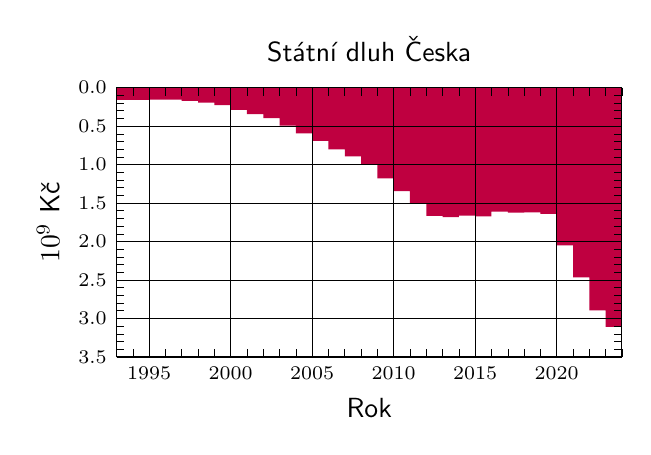
\begin{tikzpicture}
\begin{axis} [
	ybar, bar width=1, bar shift=0.5,
	width = 8cm, height = 5cm,
	title = {Státní dluh Česka},
	title style={at={(0.5,1)}},
	xlabel = {Rok},
	xmin = 1993, xmax = 2024,
	xtick = {1990,1995,...,2025},
	ylabel = {$10^9$ Kč},
	ymin = 0, ymax = 3.5,
	ytick = {0,0.5,...,3.5},
	y dir=reverse,
	grid=major, grid style={black, very thin},
	minor x tick num = 4, minor y tick num = 4,
	ticklabel style={font={\scriptsize}, /pgf/number format/.cd, 1000 sep={}},
	yticklabel style={fixed, fixed zerofill, precision=1},
	tick style={black, very thin}, tick align=inside,
	axis on top,
	]
	\addplot [draw=none, fill=purple] coordinates {%
	(1993,0.159) (1994,0.157) (1995,0.154) (1996,0.155) (1997,0.173) (1998,0.195) (1999,0.228)
	(2000,0.289) (2001,0.345) (2002,0.396) (2003,0.493) (2004,0.593) (2005,0.691) (2006,0.803)
	(2007,0.892) (2008,1.000) (2009,1.179) (2010,1.344) (2011,1.499) (2012,1.668)
	(2013,1.683) (2014,1.664) (2015,1.673) (2016,1.613) (2017,1.625) (2018,1.622)
	(2019,1.640) (2020,2.050) (2021,2.466) (2022,2.895) (2023,3.111)};
\end{axis}
\end{tikzpicture}
\end{document}
